\section{About systems and methods}
\subsection{Requirements - system}
\begin{itemize}
\item List of assumptions
\item Capture the required parameters (i.e. how to normalize the systems)
	\begin{itemize}
	\item Resonance
	\item Nonlinear elastic components
	\begin{itemize}
	\item a set of linear components for multiple modes? 
	\end{itemize}
	\end{itemize}
	
\item 
\end{itemize}
\subsection{Requirements - method}
\begin{itemize}
\item Applicable to complex system (e.g. for the designed mechanism)
\item Nondimensionlization (so that it can be used for robots with different scales)
\item Stability analysis
\item Robustness
\end{itemize}

\subsection{Remarks}
\begin{itemize}
\item Impact does not cause velocity change on runner with massless leg!
\item In SCS, to simulate massless leg, it is better to use only one body, and manipulate the relation between the contact point and the body in controller instead.
\end{itemize}

\subsection{ToDo}
\begin{itemize}
\item Rearrange/updating references for fastRunner
\item Check if the foot is sliding
\item Check optimization tools ihmc have
\begin{itemize}
\item parameter optimization tool using Gradient Decent or GA
\end{itemize}
\item Ask Cris about the parameter range/selection
\end{itemize}

\subsection{Questions}
Direction
\begin{itemize}
\item Should I exclude the gyroscopic-based stabilization? 
\item Eigen values of linearized system, Poincare map analysis, anything else I should study for the stability analysis?
\item The linkage between the control in simulation and mechanism design
	\begin{itemize}
	\item Parameters
	\item How to design a mechanism can emulate PD control?
	\end{itemize}
\end{itemize}
General Utilities 
\begin{itemize}
\item Any solver for nonlinear program IHMC used?
\item Any trajectory optimization package IHMC used?
\item Methods to get stable Reciprocating Spoked Runner?
\end{itemize}

Past simulations
\begin{itemize}
\item Why the abstract runner (in spoked runner project) can be stabilized in x direction? 
\begin{figure}[h]
\centering

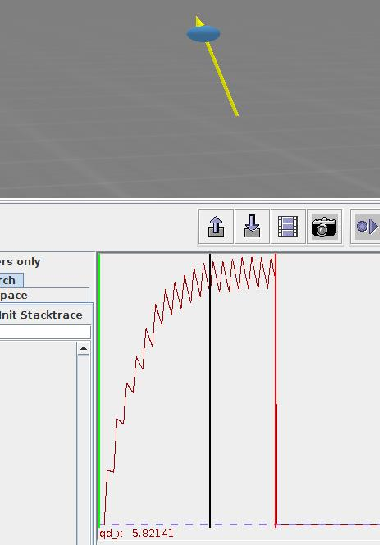
\includegraphics[scale = 0.5]{abstractRunner.pdf} 
\caption{The Abstract Runner}
%\label{fig.1DOF-Hopper}
\end{figure}
\begin{itemize}
\item The simulation setup is really robust for a large set of initial conditions/throttle angles
\item It turns out its because the added \underline{wind resistance} dissipate a lot of energies.
\end{itemize}


\item Methods to get stable Reciprocating Spoked Runner?
\item What is the line \underline{private static final long serialVersionUID } for?

\end{itemize}

\pagebreak